\documentclass[12pt,titlepage]{article}
\usepackage[margin=1.25in]{geometry}
\usepackage{graphicx,amsmath,blindtext}

%% Variables definition
\newcommand{\vSubject}{Antarmuka Pengguna}
\newcommand{\vSubtitle}{Definitions of UI/UX}
\newcommand{\vName}{Dicha Zelianivan Arkana}
\newcommand{\vNIM}{2241720002}
\newcommand{\vClass}{1i}
\newcommand{\vDepartment}{Information Technology}
\newcommand{\vStudyProgram}{D4 Informatics Engineering}

%% [START] Tikz related stuff
\usepackage{tikz}
\usetikzlibrary{svg.path,calc,shapes.geometric,shapes.misc}
\tikzstyle{terminator} = [rectangle, draw, text centered, rounded corners = 1em, minimum height=2em]
\tikzstyle{preparation} = [chamfered rectangle, chamfered rectangle sep=0.75em, draw, text centered, minimum height = 2em]
\tikzstyle{process} = [rectangle, draw, text centered, minimum height=2em]
\tikzstyle{decision} = [diamond, aspect=2, draw, text centered, minimum height=2em]
\tikzstyle{data}=[trapezium, draw, text centered, trapezium left angle=60, trapezium right angle=120, minimum height=2em]
\tikzstyle{connector} = [line width=0.25mm,->]
%% [END] Tikz related stuff

%% [START] Fancy header related stuff
\usepackage{fancyhdr}
\pagestyle{fancy}
\setlength{\headheight}{15pt} % compensate fancyhdr style
\fancyhead{}
\fancyfoot{}
\fancyfoot[L]{\thepage}
\fancyfoot[R]{\textit{\vSubject - \vSubtitle}}
\renewcommand{\footrulewidth}{0.4pt}% default is 0pt, overline for footer
%% [END] Fancy header related stuff

%% [START] Custom tabular command related stuff
\usepackage{tabularx}
\newcommand{\details}[2]{
    #1 & #2  \\
}
%% [END] Custom tabular command related stuff

%% [START] Figure related stuff
\newcommand{\image}[3][1]{
    \begin{figure}[h]
        \centering
        \includegraphics[#1]{#2}
        \caption{#3}
        \label{#3}
    \end{figure}
}
%% [END] Figure related stuff

\begin{document}
\begin{titlepage}
    \centering
    \vfill
    {\bfseries\LARGE
        \vSubject\\
        \vskip0.25cm
        \vSubtitle
    }
    \vfill
    
\includegraphics[width=6cm]{images/polinema-logo.png}
    \vfill
    {
        \textbf{Name}\\
        \vName\\
        \vskip0.5cm
        \textbf{NIM}\\
        \vNIM\\
        \vskip0.5cm
        \textbf{Class}\\
        \vClass\\
        \vskip0.5cm
        \textbf{Department}\\
        \vDepartment\\
        \vskip0.5cm
        \textbf{Study Program}\\
        \vStudyProgram
    }
\end{titlepage}

\tableofcontents
\pagebreak

\section{Definitions of UI and UX}

\subsection{User Interface (UI)}
\begin{itemize}
    \item User Interface often abbreviated as UI is an interface that is provided to the users to interact with the system
    \item Something that the users see when they use a system
    \item Can be seen with the eye since it's what the users will see upon using the system
    \item {
        There are two types of UI that are commonly used digitally, namely:
        \begin{itemize}
            \item {
                \textbf{Graphical User Interface (GUI)}
                \begin{itemize}
                    \item Used in a more modern system
                    \item Rendered as a graphical element
                    \item Has a high resolution
                    \item Can have as much detail as possible depending on the resolution of the system
                \end{itemize}
            }
            \item {
                \textbf{Terminal User Interface (TUI)}
                \begin{itemize}
                    \item Made its appearance since older system such as UNIX system or those without a modern graphical screen
                    \item Its entirety is based on text and colours manipulation
                    \item Limited to the grid system provided by the terminal
                \end{itemize}
            }
        \end{itemize}
    }
\end{itemize}

\subsection{User Experience (UX)}
\begin{itemize}
    \item User Experience often abbreviated as UX is how the user interacts with the system or product
    \item Ability of the users interacting with the system or product
    \item Cannot be seen with the eye because it's something that the users experienced throughout the system
\end{itemize}

\subsection{Conclusion}
User Interface is what the users see and User Experience is what the users feel. Both plays an important role in a system or product.

\pagebreak

\section{Good UI and UX Characteristics}

\subsection{User Interface}
\begin{itemize}
    \item Adheres to a certain laws of design
    \item Follows the accessibility (a11y) rules so that more people can use the system
    \item Looks good in the eye but shouldn't distract the users from the information given
    \item Must be able to convey informations clearly
\end{itemize}

\subsection{Examples of good UI}
\begin{itemize}
    \item {
        \textbf{Laws of UX}
        \begin{figure}[h]
            \centering
            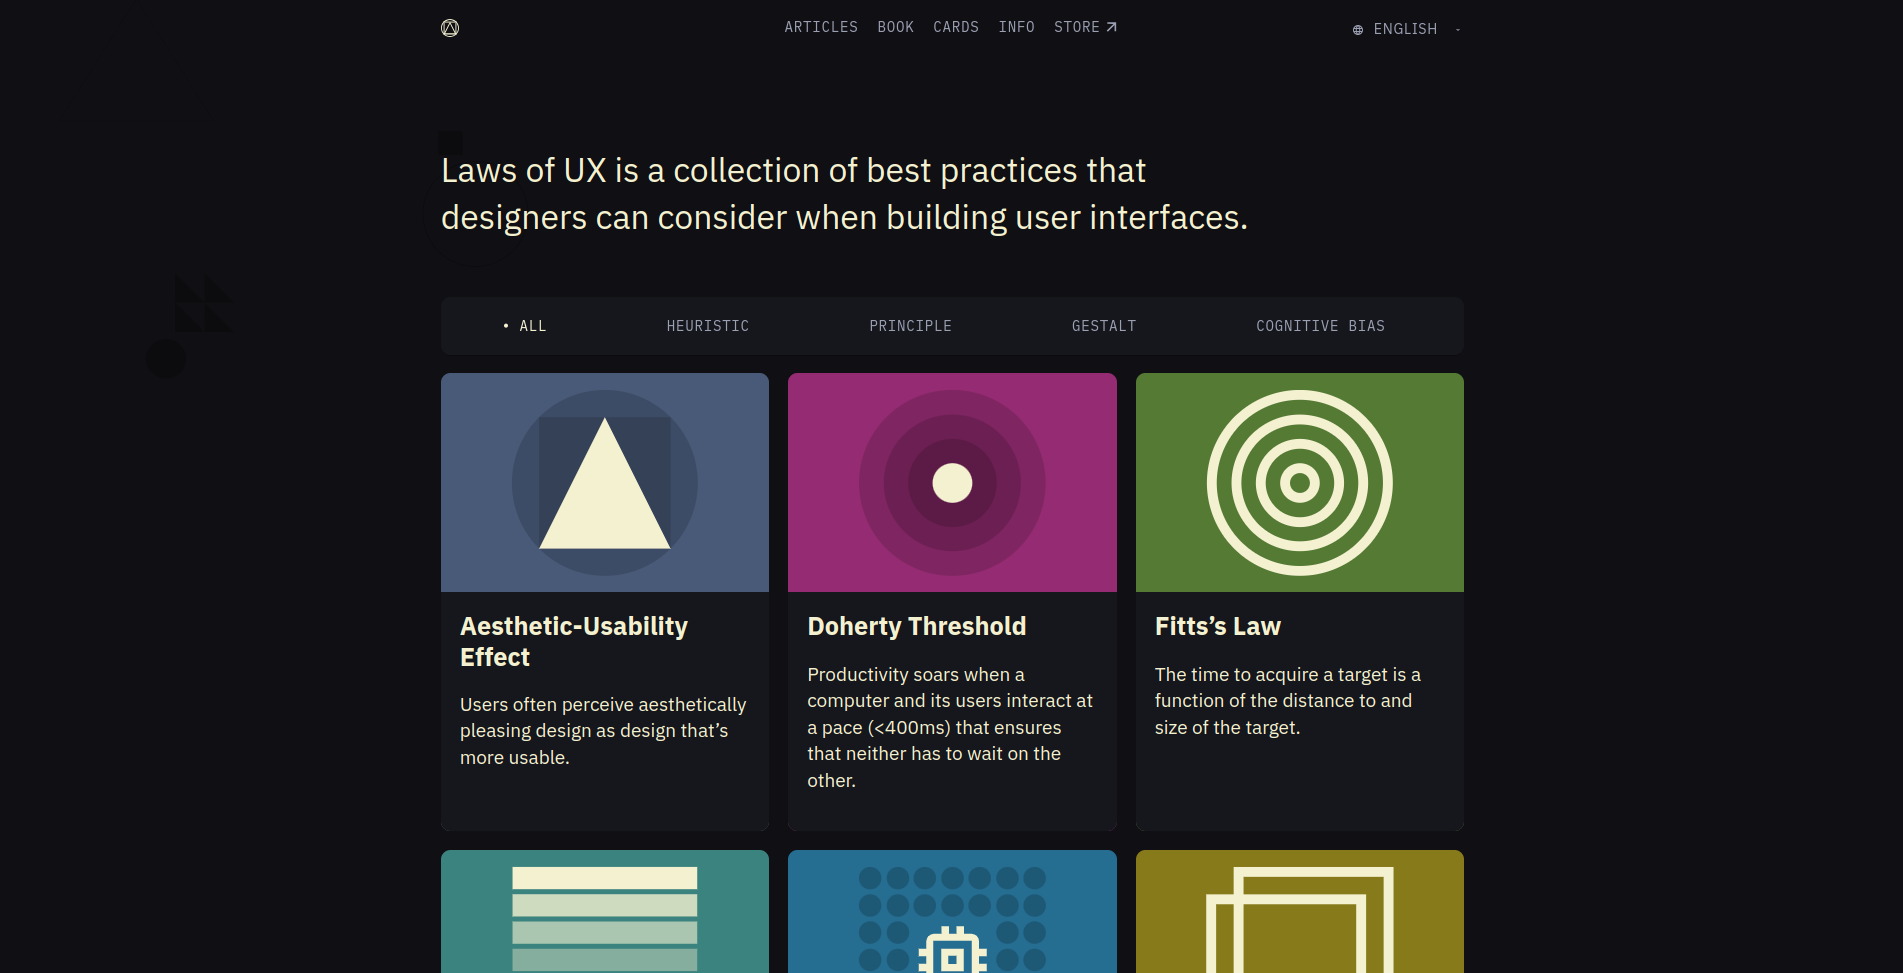
\includegraphics[width=.8\textwidth]{./images/law-of-ux.png}
            \caption{https://lawsofux.com}
        \end{figure}
        \begin{itemize}
            \item Clear in its intention, it tries to inform different laws of a good user experience
            \item Simple enough where the users can see all the informations clearly at a glance
            \item Using different colours and simple shapes to make it easier to differentiate each sections
            \item Feels clean and doesn't look cluttered
        \end{itemize}
    }
    \pagebreak
    \item {
        \textbf{Microsoft .NET}
        \begin{figure}[h]
            \centering
            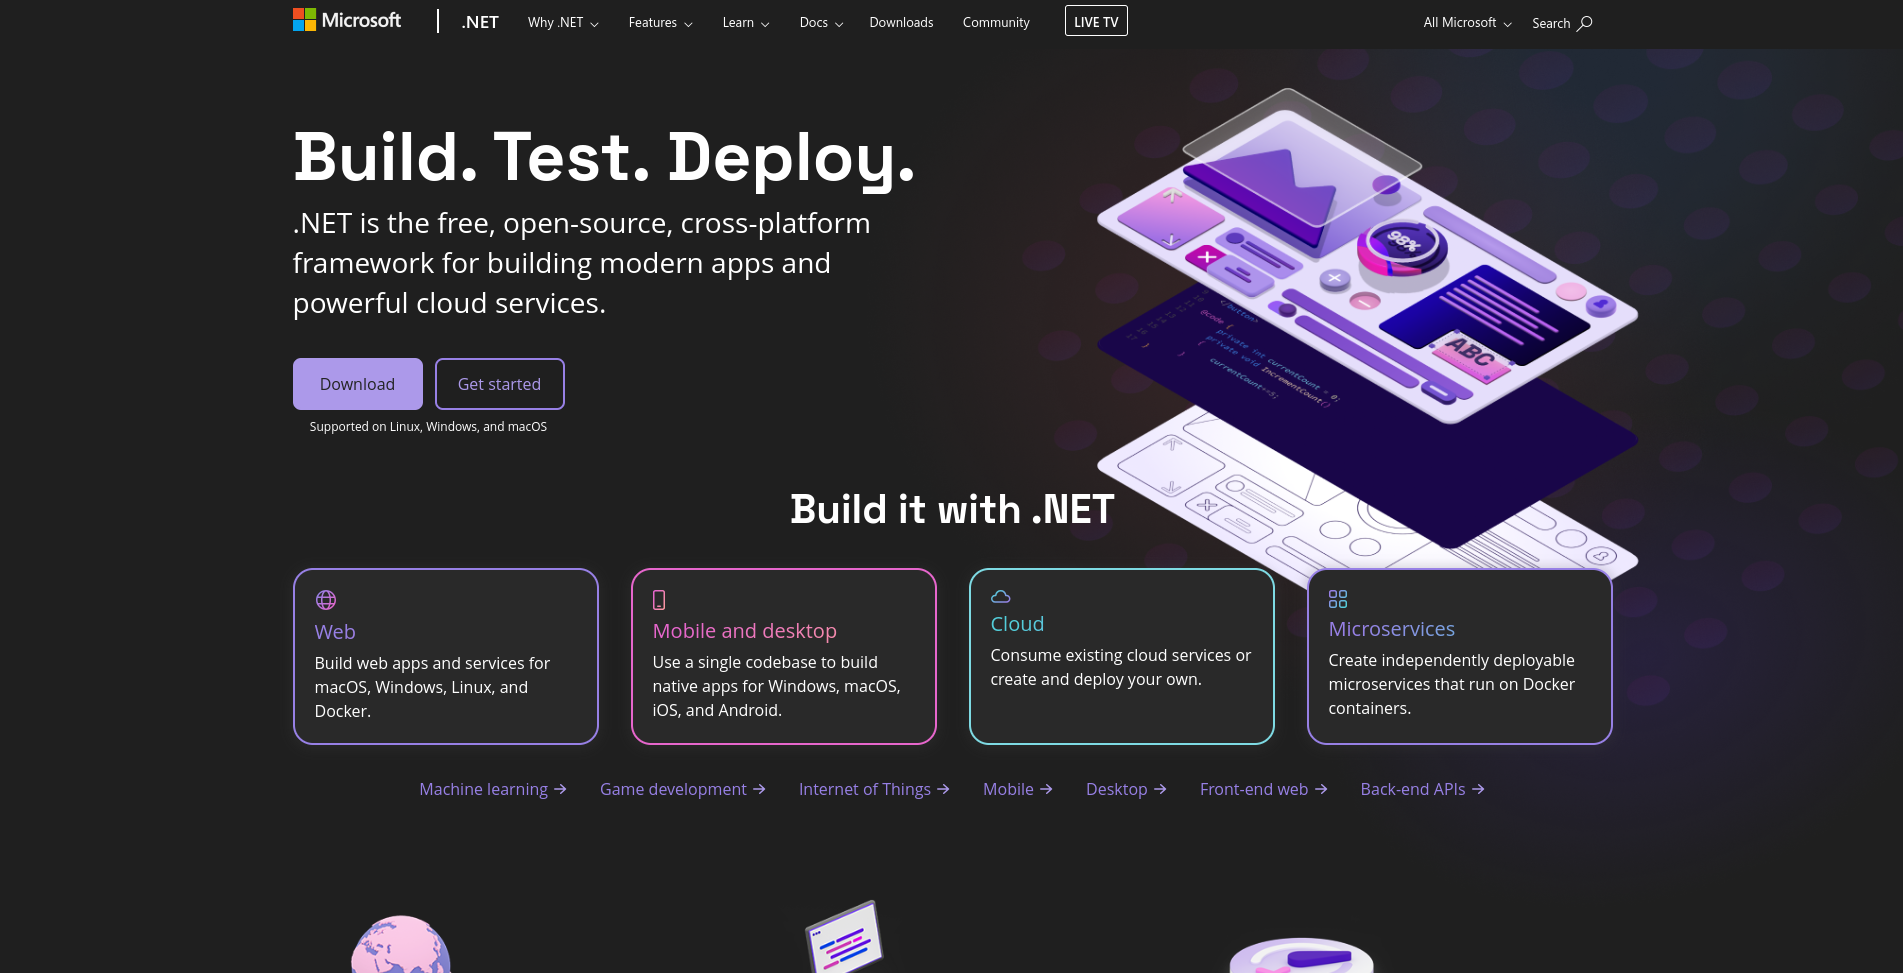
\includegraphics[width=.8\textwidth]{./images/dotnet.png}
            \caption{https://dotnet.microsoft.com}
        \end{figure}
        \begin{itemize}
            \item It has a clear tagline that attracts the attention of the user and a clear call to action button which the users can click
            \item Illustration is provided to attract the user attention, instead of just giving some boring texts
            \item Uses different colours that work with each other making it pleasing to look at
        \end{itemize}
    }
\end{itemize}

\pagebreak

\subsection{User Experience}
\begin{itemize}
    \item Adheres to a certain laws of UX
    \item Makes the interaction with the system or product feels like a breeze
    \item Does not need much explanation, or it should feel natural to the users
\end{itemize}

\subsection{Examples of good UX}
\begin{itemize}
    \item {
        \textbf{Github}
        \begin{figure}[h]
            \centering
            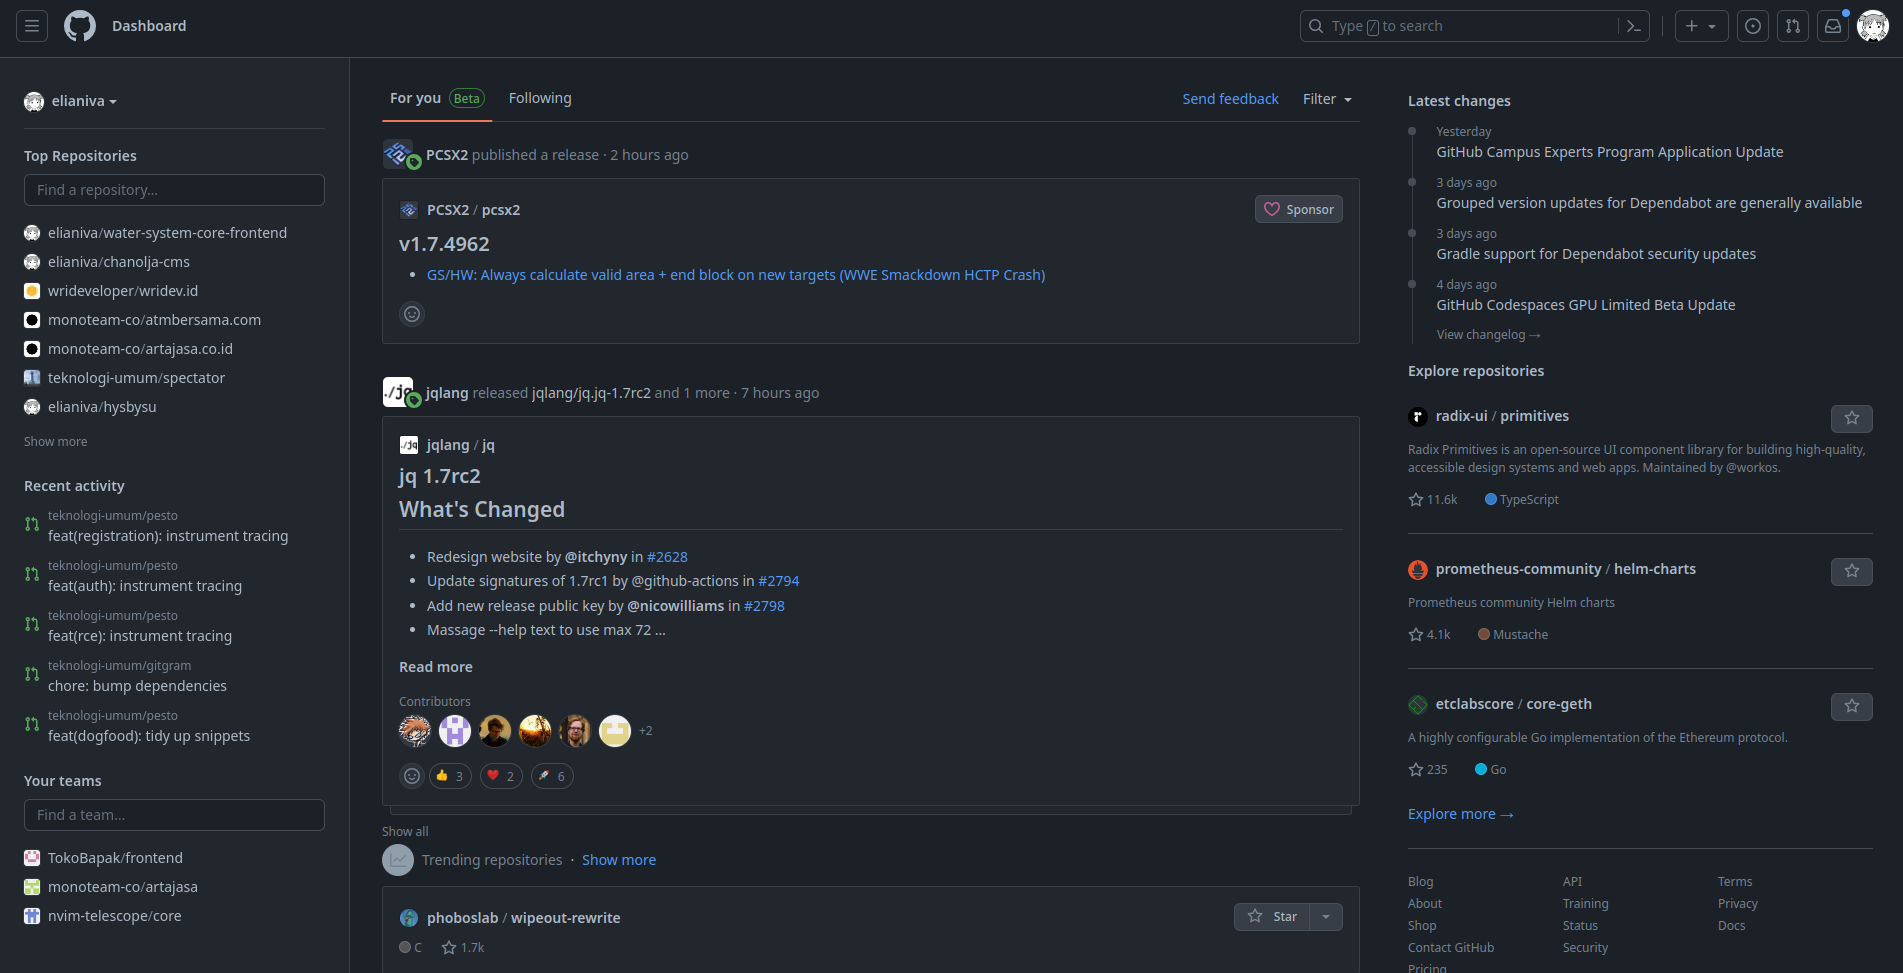
\includegraphics[width=.8\textwidth]{./images/github.png}
            \caption{https://github.com}
        \end{figure}
        \begin{itemize}
            \item Everything can be seen on a single screen yet they are all clear with their intention
            \item There's not much explanation needed since everything is self explanatory
            \item Each components have their own state when they receive interaction making it feels fluid
        \end{itemize}
    }
    \pagebreak
    \item {
        \textbf{Learn Svelte}
        \begin{figure}[h]
            \centering
            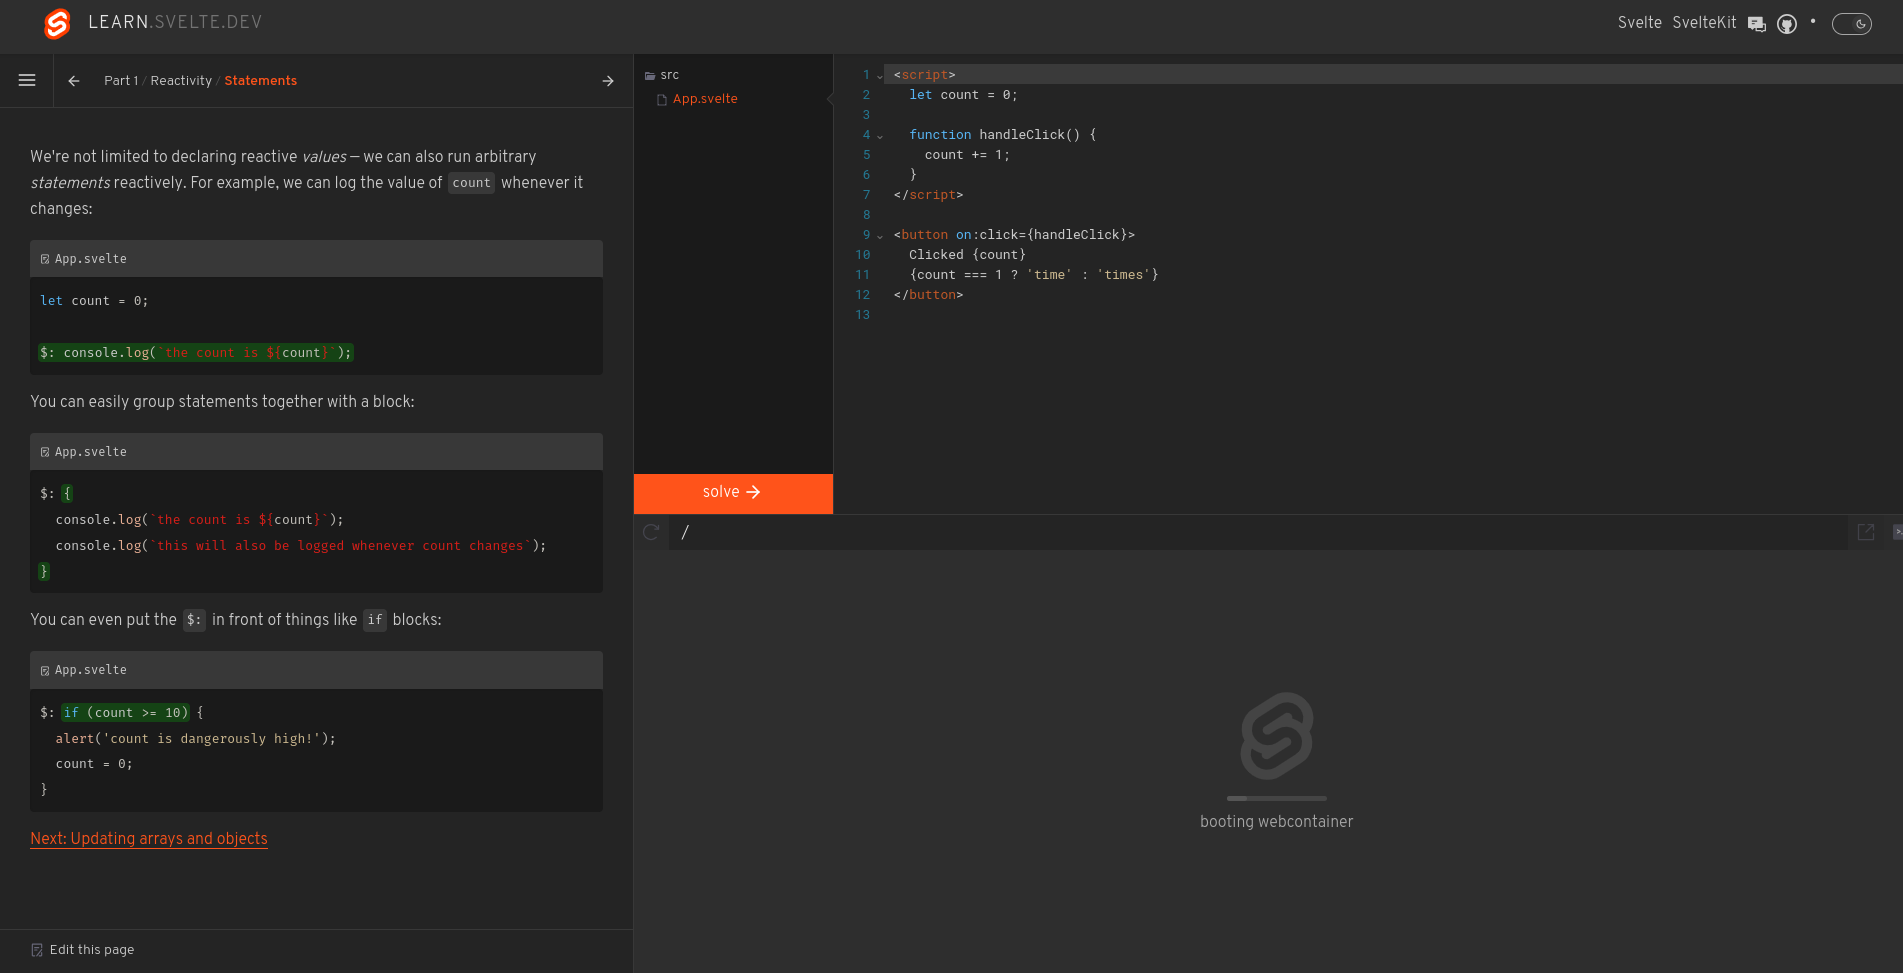
\includegraphics[width=.8\textwidth]{./images/learn-svelte.png}
            \caption{https://learn.svelte.dev}
        \end{figure}
        \begin{itemize}
            \item There's not much explanation needed since the flow of the app is clear
            \item It feels familiar to most people with at least some experience of web development
            \item Every buttons do exactly what the users think
        \end{itemize}
    }
\end{itemize}

\subsection{Conclusion}
User Interface and User Experience both have certain rules that needs to be adhered so that it provides the best experience for its users.
Having a good User Interface doesn't always mean having a good User Experience. There should be a strike of balance between the two
such that the app gives the best experience for the users. Sometimes there are tradeoff that needs to be made to make the 
UI better by sacrificing some of the UX or vice versa but that highly depends on the needs of the system or product.

\end{document}

